

Green's functions are a cornerstone of scalar and vector scattering analysis. Fundamentally, a Green's function is the impulse response of a partial differential equation, in this case, a wave equation with associated boundary conditions. The classic text on dyadic Green's functions for vector electromagnetic waves is \cite{tai1994dyadic}, along with \cite{chew1995waves,tsang1985theory}.  

Scalar and dyadic Green's functions allow us to cast scattering problems as surface or volume integral equations. These enable solutions of the scattered fields through the use of powerful numerical methods like the Method of Moments and the Conjugate Gradient FFT. In addition, Green's functions help reveal the nature of wave propagation: for example, in 3D free-space, the Green's function shows that the amplitude of waves radiated from a point source decay geometrically with distance and that information is carried undiminished in the phase of the wave.

In this chapter, we list for reference the scalar Green's function in 1D, 2D, and 3D, with far-field expressions for 2D and 3D. We provide routines for the dyadic Green's function for vector electromagnetic waves. We give the volume integral equations (VIE) for scalar and vector waves as well as the expression for the VIE under the far-field Born approximation. The Green's function is singular when evaluated at the origin, however this singularity is integrable. We give the results for the volume-integrated Green's function at singular and non-singular points which are needed when discretizing the VIE. Last, we setup the Method of Moments solution of the VIEs for both scalar and vector cases.


\section{Scalar Green's Function}

The scalar Green's function is the solution to the Helmholtz wave equation for a point source in a homogeneous medium
\eq{\nabla^2 g(\bb{r},\bb{r}') + k^2 g(\bb{r},\bb{r}') = -\delta(\bb{r}-\bb{r}')}

\noindent where $k$ is the background wavenumber, $\bb{r}$ is the observation point, and  $\bb{r}'$ is the source point. This wave equation is linear, therefore a scalar field, $\phi(\br)$, due to a distributed source, $s(\br)$, is given by the volume integral over the Green's function as, \cite{chew1995waves}
\eq{\phi(\br) = -\int g(\br,\br') s(\br') dV' \label{sourceintscalar}}

In short, the Green's function is the impulse response of the linear system that is the wave equation for homogeneous media. 

\addtocontents{toc}{\protect\setcounter{tocdepth}{1}}
\subsection{1D Scalar Green's Function}
\addtocontents{toc}{\protect\setcounter{tocdepth}{2}}

The 1D free-space scalar Green's function is 
\eq{g(x,x')  = \dfrac{i}{2k} e^{ik\vert x-x' \vert}}

\noindent where $x$ is the observation point, $x'$ is the source point, and $k$ is background wavenumber. This has no far-field approximation because there is no wave spreading in 1D.   

\addtocontents{toc}{\protect\setcounter{tocdepth}{1}}
\subsection{2D Scalar Green's Function}
\addtocontents{toc}{\protect\setcounter{tocdepth}{2}}

The 2D free-space scalar Green's function is 
\eq{g(\boldsymbol{\rho},\boldsymbol{\rho}') = \dfrac{i}{4} H_0^{(1)}\left(k \vert \boldsymbol{\rho} - \boldsymbol{\rho}'\vert\right) }

\noindent where $\boldsymbol{\rho}$ is the observation point, $\boldsymbol{\rho}'$ is the source point, $k$ is the background wavenumber and $H_0^{(1)}$ is the Hankel function, \cite{chew1995waves}. This is the solution to the Helmholtz wave equation in a homogenous medium due to 2D line source. This has far-field approximation 
%\eq{g(\boldsymbol{\rho},\boldsymbol{\rho}') \approx \dfrac{i}{4} \sqrt{\dfrac{2}{\pi k \rho }} e^{k\rho - \frac{n\pi}{2} - \frac{\pi}{4} }}
\eq{g(\boldsymbol{\rho},\boldsymbol{\rho}') \approx  \sqrt{\dfrac{1}{8 \pi k \rho }} e^{i\pi/4 } e^{i k\rho } e^{-ik \hat{\boldsymbol{\rho}}\cdot\boldsymbol{\rho}' }}

This shows that fields decay like $1/\sqrt{\rho}$ in 2D. 

\addtocontents{toc}{\protect\setcounter{tocdepth}{1}}
\subsection{3D Scalar Green's Function}
\addtocontents{toc}{\protect\setcounter{tocdepth}{2}}

The 3D free-space scalar Green's function is 
\eq{g(\br,\br') = \dfrac{e^{ik\vert \br - \br' \vert}}{4\pi \vert \br - \br' \vert}}
\noindent where $k$ is the background wavenumber, $\br'$ is the source point, $\br$ is the observation point.  This is the solution to the Helmholtz wave equation due to a point source in three dimensions.  The far-field approximation is 
\eq{g(\br,\br') \approx \dfrac{e^{ikr}}{4\pi r} e^{-ik \hat{\br}\cdot\br' } }

This shows the classic result that fields decay like $1/r$ in 3D. 

\section{Dyadic Green's Function}

The free-space electric field dyadic Green's function satisfies the vector wave equation \cite{chew1995waves,tai1994dyadic}
\eq{\nabla \times \nabla \times  \overline{\bb{G}}(\br,\br') - k^2 \overline{\bb{G}}(\br,\br') = \overline{\bb{I}} \delta(\br - \br')}

\noindent where $\overline{\bb{I}}$ is the identity dyad. This is often notated $\overline{\bb{G}}_e(\br,\br')$ to distinguish it from the magnetic field dyadic Green's function.  The electric field due to a distributed current density $\bb{J}(\br)$ is given by 

\eq{\bb{E}(\br) = i\omega\mu\int \G{} \cdot \bb{J}(\br') dV'  \label{evolintj}}

The dyadic Green's function is given by 
\begin{equation}
 \overline{\bb{G}}(\br,\br') = \left[\overline{\bb{I}} + \dfrac{1}{k^2} \nabla\nabla \right] \dfrac{e^{ik\vert \br - \br' \vert}}{4\pi \vert \br - \br' \vert} \label{dgreens}
 \end{equation}

\noindent where $k$ is the background wavenumber, $\br'$ is the source point, $\br$ is the observation point, and 

\begin{equation}
\nabla = \dfrac{d}{dx} \hat{x} + \dfrac{d}{dy} \hat{y}  + \dfrac{d}{dz} \hat{z} 
\end{equation}


Writing out \eqref{dgreens},
\begin{equation}
\overline{\bb{G}}(\br,\br')  = \thbth
{k^2 + \dfrac{\partial^2}{\partial x^2}}{\dfrac{\partial^2}{\partial x\partial y}} {\dfrac{\partial^2}{\partial x\partial z}} 
{\dfrac{\partial^2}{\partial y\partial x}} {k^2 + \dfrac{\partial^2}{\partial y^2}} {\dfrac{\partial^2}{\partial y\partial z}} 
{\dfrac{\partial^2}{\partial z\partial x}} {\dfrac{\partial^2}{\partial z\partial y}} {k^2 + \dfrac{\partial^2}{\partial z^2}}
\dfrac{e^{ik\vert \br - \br' \vert}}{4\pi k^2 \vert \br - \br' \vert}
\end{equation}

The dyadic Green's function is symmetric with six unique dyadic components. In Cartesian coordinates the components are 
\begin{eqnarray}
G_{xx} &=& (1+c_1(x-x')^2+c_2)c_3 \\
G_{yy} &=& (1+c_1(y-y')^2+c_2)c_3 \\ 
G_{zz} &=& (1+c_1(z-z')^2+c_2)c_3 \\
G_{xy} &=& c_1(x-x')(y-y')c_3 \\
G_{xz} &=& c_1(x-x')(z-z')c_3 \\ 
G_{yz} &=& c_1(y-y')(z-z')c_3 
\end{eqnarray}

\noindent where
\begin{eqnarray}
r &=& \vert \br - \br' \vert \\
c_1 &=& -\dfrac{1}{r^2} - \dfrac{3i}{k r^3} + \dfrac{3}{k^2 r^4} \\
c_2 &=& \dfrac{i}{kr} - \dfrac{1}{k^2r^2} \\
c_3 &=& \dfrac{e^{ikr}}{4\pi r}
\end{eqnarray}

The far field approximation of the dyadic Green's function is 
\begin{equation} \overline{\bb{G}}(\br,\br') \approx \left[\overline{\bb{I}} - \hat{r}\hat{r}\right] \dfrac{e^{ikr}}{4\pi r} e^{-ik \hat{\br}\cdot\br' \label{dyadicGff}} 
 \end{equation}
 
\noindent where $\overline{\bb{I}} - \hat{r}\hat{r} = \hat{\theta}\hat{\theta} + \hat{\phi}\hat{\phi}$ in spherical coordinates.  The curl of the dyadic Green's function is used in surface integral equations and is given by 
\eq{\curl \G{} = \nabla g(\br,\br') \times \overline{\bb{I}}}

Written out it is 
\begin{equation}
\curl \G{} = \thbth
{0}{-\dd{}{z} } {\dd{}{y} } 
{\dd{}{z} } {0} {-\dd{}{x}}
{-\dd{}{y} } {\dd{}{x}} {0}
\dfrac{e^{ik\vert \br - \br' \vert}}{4\pi   \vert \br - \br' \vert}
\end{equation}



The unique components, to within a sign, are 
\begin{eqnarray}
\left[\curl \G{}\right]_{xy}  &=& -(z-z') f(r) \\
\left[\curl \G{}\right]_{xz}&=& (y-y') f(r) \\ 
\left[\curl \G{}\right]_{yz}&=& - (x-x') f(r) \\
f(r) &=& (i k r-1) \dfrac{e^{i k r}}{4 \pi r^3} 
\end{eqnarray}

A useful property is
\eq{\curl \G{}= -\nabla'\times \G{} \label{dyadicGreenscurlprime}}

\clearpage
\newpage
The routine \texttt{dyadicGreens} takes as input the wavenumber $k$, and components of the difference vector $\br - \br'$ in Cartesian coordinates and returns the six unique matrix entries of the dyadic Green's function.  The routine \texttt{curlDyadicGreens} takes the same inputs and returns the six matrix entries of the curl of the dyadic Green's function. These are straight computations. No provisions are made for the singularity.  

{\footnotesize
\VerbatimInput{\code/GreensFunctions/dyadicGreens.m}
}

{\footnotesize
\VerbatimInput{\code/GreensFunctions/curlDyadicGreens.m}
}

\clearpage
\newpage
\section{Volume Integral Equation}

The volume integral equation (VIE) formulates the scattering solution of a heterogeneous distribution of material in terms of the Green's function for homogenous media, \cite{chew1995waves}. The VIE applies to both scalar and vector problems and is the basis of many numerical solvers, such as the Method of Moments. It serves as the basis for many inverse scattering algorithms. 

\subsection{Scalar VIE}
Start with the Helmholtz wave equation where the wavenumber of the medium is a function of position
\eq{\nabla^2 \phi(\br) + k^2(\br) \phi(\br) = s(\br)}

This equation is classified as an inhomogeneous, linear, second-order partial differential equation with non-constant coefficients. Assuming that the material object is bounded and sits in a background medium with wavenumber $k_b$, the next step is to add and subtract $k_b^2$ from the object as
\eq{\nabla^2 \phi(\br) + (k^2(\br) + k_b^2 - k_b^2)\phi(\br) = s(\br)}

Keeping the factor of $+k_b^2$ on the LHS and moving everything else to the RHS 
\eq{\nabla^2 \phi(\br) +  k_b^2\phi(\br) = s(\br) -  (k^2(\br) - k_b^2)\phi(\br) }

The LHS is the wave equation for the homogenous background which is sourced by everything on the RHS. The field solution is given by integrating the RHS with the free-space Green's function per \eqref{sourceintscalar} 
\eq{\phi(\br) = -\int g(\br,\br') s(\br') dV' +  \int g(\br,\br') (k^2(\br') - k_b^2)\phi(\br') dV'}

The first term on the RHS is the field due to the source in the absence of the object. This is the incident field, $\phi_{inc}(\br)$. The scalar VIE is then written
\eq{\phi(\br) = \phi_{inc}(\br) +  \int g(\br,\br') O(\br') \phi(\br') dV' \label{scalarVIE}}

\noindent where the object function, $O(\br) = k^2(\br) - k_b^2 $, is the contrast of the object relative to the background.  This is a Fredholm integral equation of the second kind because the total field, $\phi(\br)$, appears inside and outside the integral. The integral term is defined as the scattered field. The scattered field modifies the incident field to give the total field. The scattered field exists inside and outside the object, even though the scattered field depends on the total field in the object. We can express this idea simply as
\eq{\phi(\br) = \phi_{inc}(\br) +  \phi_{sca}(\br) }

In experiment, only the incident and total fields can be measured directly using sources and receivers placed away from the object. The incident field is measured in the absence of the object and the total field measured in the presence of the object. The scattered field is obtained by subtracting the measured incident and total fields. For situations in which the object cannot be removed, the incident field has to be predicted using a model of the source and receiver. %In order to make the measurements and computations of the VIE consistent, the total field solution should be obtained using an incident field from the same source model.

\subsection{Vector VIE}

The vector VIE is derived from the vector wave equation in the same way as the scalar VIE is derived from the Helmholtz wave equation. The vector wave equation for the total electric field in an isotropic inhomogeneous non-magnetic dielectric medium is \cite{chew1995waves}
\eq{\nabla \times \nabla \times  \bb{E}(\br) - k^2(\br) \bb{E}(\br) = i\omega\mu_o \bb{J}(\br)}

Adding and subtracting the background wavenumber, $k_b^2$, to $k^2(\br)$, rearranging, and integrating the source terms with the free-space dyadic Green's function, the vector VIE is 
\eq{\bb{E}(\br) = \bb{E}_{inc}(\br) + \int \G{} \cdot O(\br') \bb{E}(\br') dV' \label{vectorVIE} }

$\bb{E}_{inc}(\br)$ is the incident field in the absence of the object and can be computed with \eqref{evolintj} given a the source distribution $\bb{J}(\br)$. The object function is 
\ea{O(\br) &=& k^2(\br) - k_b^2 \\
\ &=& k_o^2 \left(  \delta\epsilon_r(\br) + i\dfrac{\delta \sigma(\br)}{\epsilon_o \omega}\right) \label{objectfunction} \\
\delta\epsilon_r(\br) &=& \epsilon_r(\br) - \epsilon_{rb} \\
\delta \sigma(\br) &=& \sigma(\br) - \sigma_b}

\noindent where $k_b = \omega\sqrt{\mu_o\epsilon_b}$ is the background wavenumber, $\epsilon_b$ is the background permittivity, and $k_o^2 = \omega^2\mu_o\epsilon_o$ is the lossless free-space background wavenumber. The complex permittivity is, generally, $\epsilon = \epsilon_o(\epsilon_r + i\sigma/(\omega\epsilon_o))$, where $\epsilon_r$ is the real part, $\sigma$ is the conductivity, and $\omega$ the natural frequency, \cite{chew1995waves}. Using this, one can derive the functions $\delta\epsilon(\br)$ and $\delta \sigma(\br)$ which are the permittivity and conductivity contrasts relative to the background. Note, the dyadic Green's function is evaluated with the background wavenumber $k_b$. 

Using 
\eq{\bb{E}(\br) = \bb{E}_{inc}(\br) + \bb{E}_{sca}(\br)}

the scattered field is given by the integral term
\eq{\bb{E}_{sca}(\br)=  \int \G{} \cdot O(\br') \bb{E}(\br') dV' \label{vie}}

%\noindent where the object function is
%\ea{O(\br) &=& k^2(\br) - k_b^2 \\
%\ &=& k_o^2 \left(  \delta\epsilon(\br) + i\dfrac{\delta \sigma(\br)}{\epsilon_b \omega}\right) \label{objectfunction} \\
%\epsilon_b \delta\epsilon(\br) &=& \epsilon(\br) - \epsilon_b \\
%\delta \sigma(\br) &=& \sigma(\br) - \sigma_b}
%
%\noindent where $k_b = \omega\sqrt{\mu_b\epsilon_b}$ is the background wavenumber, $k_o^2 = \omega^2\mu_o\epsilon_b$ is the lossless background wavenumber, $\epsilon_b = \epsilon_o \epsilon_{rb}$ is the real part background permittivity. The functions $\delta\epsilon(\br)$ and $\delta \sigma(\br)$ are the permittivity and conductivity contrast relative to the background. In general, the complex permittivity is given by $\epsilon = \epsilon_o(\epsilon_r + i\sigma/(\omega\epsilon_o))$, where $\epsilon_r$ is the real part, $\sigma$ is the conductivity, and $\omega$ the natural frequency, \cite{chew1995waves}.


%  The background dyadic Green's function is

%\eq{\G{} = \left[ \overline{\bb{I}} + \dfrac{\nabla'\nabla'}{k^2} \right] \dfrac{e^{ik \vert \br - \br'\vert}}{4\pi  \vert \br - \br'\vert}  }

%and 
%\eq{k^2 = k_o^2\left(1 + i \dfrac{\sigma_b}{\epsilon_b \omega} \right)}

%Using \eqref{dyadicGff}, the far-field approximation of the Green's function in the scattered field direction is 
%\eq{\G{} \approx \left[ \overline{\bb{I}}  - \hat{r}\hat{r} \right] \dfrac{e^{ikr}}{4\pi r} \exp(-i \bb{k}_s\cdot\br' ) \label{dgff} } 

%\noindent where $\bb{k}_s$ is the wave vector in the scattered or radial direction. % In spherical coordinates $\overline{\bb{I}}  - \hat{r}\hat{r} = \hat{\theta}\hat{\theta} + \hat{\phi}\hat{\phi}$.


\section{Far-field Born Approximation}
\label{bornapprox}

We give the classic expression for the vector field volume integral equation under the far-field Born approximation. The Born approximation refers to any instance in which the total field in an object is approximated by the incident field. In the far-field Born approximation, the VIE is simplified with three assumptions:
\begin{enumerate}
\item The Born approximation is made for the total field in the object: $\bb{E}(\br) = \bb{E}_{inc}(\br)$,
\item The incident field is a plane wave, $\bb{E}_{inc}(\br) = \bb{E}_i\exp(i \bb{k}_i \cdot \br)$,
\item The far-field dyadic Green's function, \eqref{dyadicGff}, is used in the scattered field direction, $\bb{k}_s$:
\eq{\G{} \approx \left[ \overline{\bb{I}}  - \hat{r}\hat{r} \right] \dfrac{e^{ikr}}{4\pi r} e^{-i \bb{k}_s\cdot\br'} \nonumber } 
\end{enumerate}

Substituting these into \eqref{vie}, the far-field Born approximation for the VIE is 
%\eq{\bb{E}_{sca}(\br)=  \int \left[ \overline{\bb{I}}  - \hat{r}\hat{r} \right] \dfrac{e^{ikr}}{4\pi r} \exp(-i \bb{k}_s\cdot\br' ) \cdot O(\br') \bb{E}_i \exp(i \bb{k}_i \cdot \br')  dV' }
\eq{\bb{E}_{sca}(\br)\approx  \dfrac{e^{ikr}}{4\pi r} \left[ \overline{\bb{I}}  - \hat{r}\hat{r} \right] \cdot  \bb{E}_i  \int O(\br') e^{i (\bb{k}_i-\bb{k}_s) \cdot \br'}  dV'  \label{baesca} }

The integral is the 3D Fourier transform of the object function, $O(\br)$, \eqref{objectfunction}, in the wave vector difference domain. There is no multiple scattering or depolarization due to scattering: the incident polarization is simply projected onto the scattered field polarizations based on the geometry of the source and observer. The Born approximation is a weak assumption because it assumes that the total field solution is unaffected by the object. It is only valid when the objects are very small compared to the wavelength or have very low contrast. This expression is the foundation of the $k$-space mapping between source/receiver direction pairs and the Fourier spectral components of the object, and is the basis of diffraction tomography imaging algorithms, \cite{devaney1984geophysical,chew1995waves}. 



\section{Volume-Integrated Free-space Green's Functions}
\label{volintfsgf}
The VIEs need to be discretized for numerical computation, for example, in the Method of Moments or Conjugate Gradient FFT. The discretization can be done with cubic voxels that are small enough so that the total field and object are considered constant in the voxel after which only the Green's function has to be integrated over the voxel. The Green's function, and therefore the integrand, will be singular whenever $\br = \br'$. However, the singularity is integrable in both the scalar and vector cases. When $\br \ne \br'$, the volume-integrated Green's function takes a different but constant value. The solutions to integrating the singularity are analytical if the voxel is spherical, therefore, cubic voxels are replaced with volume-equivalent spheres. The derivations are  involved (e.g., principal values, exclusion volumes), but the result is a straightforward replacement of the continuous VIE with a sum over discrete cells and appropriate scale factors.

\addtocontents{toc}{\protect\setcounter{tocdepth}{1}}
\paragraph{3D Voxel Integration}
\addtocontents{toc}{\protect\setcounter{tocdepth}{2}}

From \cite{chew1995waves,gao2005analytical}, the volume-integrated 3D scalar and dyadic Green's functions at the singular points are 
\eq{g(\br = \br') \rightarrow \dfrac{1}{k_b^2} \left(-1 + (1-ik_b a) e^{ik_b a}\right) \label{singint}}
and
\eq{\bb{G}(\br=\br') \rightarrow \dfrac{1}{k_b^2} \left( -1 + \dfrac{2}{3} (1 - i k_b a) e^{i k_b a}\right) \overline{\bb{I}} \label{singintvec}} 
\noindent where $a$ is the radius of the volume-equivalent sphere of the cubic voxels and $k_b$ is the background wavenumber. These values replace the voxel-integrated Green's function at the singularity and no factor of differential volume is needed. The source, object, or total field is assumed constant at the singular point and sampled directly. When substituted into the VIE, the factor of $1/k_b^2$ will cancel the dimensions of the object function, $O(\br)$, which has dimensions of $k_b^2$, leaving only the dimensions of the total field. 

For non-singular points, assuming that the observation point is outside of the sphere surrounding the singular point, the Green's function, source, object or total field is sampled directly, but the differential volume is replaced with, \cite{gao2005analytical},  
\eq{\Delta V = \dfrac{4\pi a}{k_b^2} \left( \dfrac{\sin(k_b a)}{k_b a} - \cos(k_b a)\right) \label{voxelint}}

This applies to both scalar and dyadic cases. Note, $\Delta V$ has dimensions of length cubed. To gain more physical insight, we can rewrite this as
\eq{\Delta V = \dfrac{4}{3}{\pi a^3} \left( 3 \dfrac{\sin(k_b a) - k_b a \cos(k_b a)}{(k_b a)^3}\right)}

The oscillating term in parentheses accounts for the coherence/decoherence of summing the phase term of the Green's function over the sphere. It has a maximum value of 1 when $k_b a \rightarrow 0$. This means that as the voxel size decreases, the integration of the Green's function becomes less important, and the volume element can be approximated just as well with the cubic volume. This expression is nearly identical to that derived in Section \ref{sec:volumephaseint} for the volume phase integral over a sphere.



\addtocontents{toc}{\protect\setcounter{tocdepth}{1}}
\paragraph{2D Voxel Integration}
\addtocontents{toc}{\protect\setcounter{tocdepth}{2}}
When the volume integrals are 2D, and discretized with squares, the singular point of the 2D scalar Green's function integrates to, \cite{gao2005analytical},
\eq{g(\boldsymbol{\rho} = \boldsymbol{\rho}') \rightarrow -\dfrac{1}{k_b^2} + \dfrac{i\pi a}{2k_b} H_1^{(1)}(k_ba) }

This has dimensions of the length squared, which cancels the dimensions of the object function in the VIE. The differential surface element is replaced with
\eq{\Delta S = \dfrac{2\pi a}{k_b} J_1(k_ba) \label{voxelsurfint}}

\noindent where $a$ is the radius of the area-equivalent disk, $k_b$ is the background wavenumber and $\Delta S$ has dimensions of length squared. Similar to \eqref{voxelint}, \eqref{voxelsurfint} is equal to the area of the voxel when $k_b a \rightarrow 0$.

The routine \texttt{volintGreens} returns the volume-integrated Green's function and discrete volume element for the cases above. It takes as input the radius of the circular or spherical voxel, $a$, the background wavenumber, $k_b$, and a string switch with three options: \texttt{'2D'} for scalar 2D, \texttt{'3D'} for scalar 3D, or \texttt{'dyadic'} for the 3D dyadic version. Often $a$ and $k_b$ are constant in a given VIE discretization, but the routine is vectorized to take arrays of values.

{\footnotesize
\VerbatimInput{\code/GreensFunctions/volintGreens.m}
}

\clearpage
\newpage


\section{Method of Moments}

The VIEs provide a framework for solving for the total field solution inside an inhomogeneous distribution of material and then using the total field solution to predict the scattered field at points away from the object. In their continuous forms, the VIEs are nonlinear functions of the total field. The Method of Moments (MoM, or Moment Method) is a procedure to discretize the VIEs in order to cast the scattering problem as a system of linear equations to which linear algebra algorithms can be applied. In general, for an accurate solution an object must be discretized better than $\lambda/10$ for the wavelength in the highest dielectric constant in the object. 

\subsection{Pulse Basis Function}
The simplest discretization of the VIE are pulse basis functions. The object and field are sampled with non-overlapping cubic voxels, where it is assumed the the object and field are constant in each voxel. The object function is approximated as 
\eq{O(\br) \approx \sum_{n} O_{n} \delta_{n}(\br)}
\eq{\delta_{n}(\br) = \begin{cases} 1, \quad \br \in \textrm{voxel } n \\
0, \quad \textrm{otherwise}  \end{cases} \label{pulsebf}
}

\noindent where $n$ indexes the set of voxels in 2D or 3D.  

\subsection{Scalar MoM} 

Using the pulse basis function, two versions of the MoM for the scalar VIE can be derived. The first is written as a solution for the total field. This is useful for inverse scattering problems when the total field is needed separate from the object.  The second version is written in terms of the induced source, or contrast source, \cite{van1997contrast}. The induced source is advantageous if a) the total field is not needed, b) there are many objects to simulate, because  the object only appears the diagonal of the MoM matrix, or c) only the scattered field away from the object needs to be computed.

\paragraph{Total Field}

Substituting the pulse basis function discretization of the object, \eqref{pulsebf}, into the VIE, \eqref{scalarVIE}
\eq{\phi(\br) = \phi_{inc}(\br) +  \sum_{n} \int g(\br,\br') O_{n} \delta_{n}(\br')\phi(\br') dV' }

Next, the incident and total fields are assumed constant in each voxel and the fields outside of the integral are sampled as the same points as those in the integrand, but indexed separately
\eq{\phi(\br_m) = \phi_{inc}(\br_m) +  \sum_{n} \int g(\br_m,\br') O_{n} \delta_{n}(\br')\phi(\br_n) dV' }

The last step is to integrate the Green's function over the voxels. Using the results of Section \eqref{volintfsgf}, this becomes
\eq{\phi_m = \phi_{inc,m} +  \sum_{n} g_{mn} O_{n} \phi_n \label{phidiscrete} }
\eq{g_{mn} = \begin{cases} g(\bb{r}_m,\bb{r}_n) \Delta V, \quad m \neq n\\
g(\bb{r}_m=\bb{r}_n), \qquad m = n\end{cases}}

\noindent where $\Delta V$ is given by \eqref{voxelint}, and the integration over the singular point is given by \eqref{singint}, where the cubic voxels have been replaced by volume-equivalent spheres. The same procedure applies in 2D.  

Writing \eqref{phidiscrete} in matrix notation 
\eq{\left(\bb{I} - \bb{G} \bb{O} \right)\boldsymbol{\phi}  = \boldsymbol{\phi}_{inc} \label{momscalarfield}}

\noindent where $\bb{I}$ is the identity matrix, $\boldsymbol{\phi}$ is the vector of unknown total field values at each voxel, $\boldsymbol{\phi}_{inc}$ is the known incident field at the same voxels, $\bb{G}$ is a full, symmetric matrix containing the Green's function values, and $\bb{O}$ is a diagonal matrix containing the values of the object function at each voxel. The right multiplication of $\bb{O}$ to $\bb{G}$ makes the final matrix asymmetric for inhomogeneous objects.  A zero-contrast voxel has the effect of zeroing-out a column of the Green's function matrix, but the identity matrix makes the overall MoM matrix safe to invert. This last feature is one reason why the total field formulation is useful for iterative inverse scattering problems where the object contrast is not known ahead of time.  Put another way, when the object contrast is zero, the total field solution is not necessarily zero. 

\paragraph{Induced Source}

The induced source, or contrast source, is defined as the product of the object contrast and the total field
\eq{w(\bb{r}) = O(\br) \phi(\br)}

Multiplying \eqref{scalarVIE} by $O(\br)$, the VIE can be written
\eq{w(\br) = w_{inc}(\br) +  O(\br) \int g(\br,\br') w(\br') dV' \label{wvie}}

Applying the MoM, we get the linear system
\eq{\left(\bb{I} - \bb{O} \bb{G}\right) \boldsymbol{w}  = \boldsymbol{w}_{inc} \label{wmomvie}}

This is similar to \eqref{momscalarfield} where the LHS matrix is asymmetric.  Alternatively, taking \eqref{wvie} or \eqref{wmomvie} and multiplying through by $1/O(\br)$ we can write
\eq{\left(\bb{O}^{-1} - \bb{G}\right) \boldsymbol{w}  = \boldsymbol{\phi}_{inc} \label{mominducediag}}

In this form the object only appears along the diagonal which makes the entire LHS matrix symmetric. This is similar to the more standard representation of the MoM, \cite{peterson1998computational}, when it is given in terms of the impedance matrix, the induced current, and the incident field. In \eqref{mominducediag}, if the object contrast of a voxel is zero, then the diagonal matrix element is infinite. The matrix either has to be reformed to exclude the rows and columns of the zero contrast, or a large numerical value needs to be substituted for the inverse contrast. In general, \eqref{mominducediag} is useful for simulating sparse dielectric objects, such as snow aggregates or vegetation, because the MoM matrix only needs to contain the interactions between voxels that have non-zero contrast. 

\begin{figure}[H] 
   \centering
      \begin{tabular}{cc}
     \subfigure{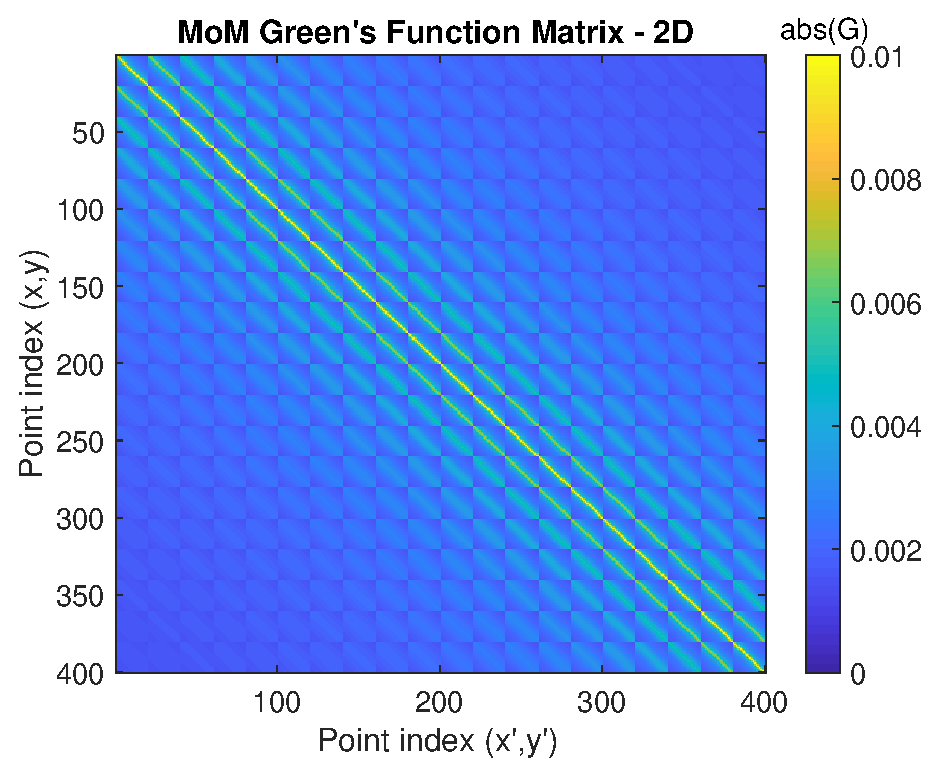
\includegraphics[width=2.5in]{GreensFunctions/Figures/green2d}}
     \subfigure{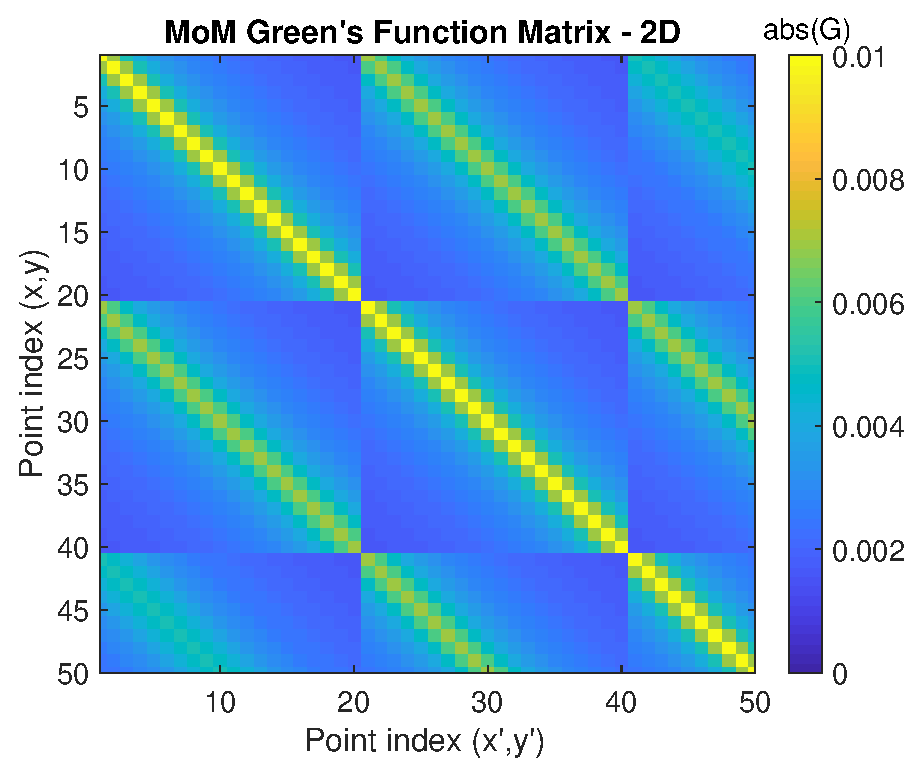
\includegraphics[width=2.5in]{GreensFunctions/Figures/green2d_v2}}
  \end{tabular}
  \label{}
\caption{2D scalar Green's function matrix, $\bb{G}$. Left: absolute value of the elements for the full matrix for a 20 $\times$ 20 grid of points sampled at $\lambda/10$ (total size $2\lambda \times 2 \lambda$). Right: zoom in. The blocks are due to vectorizing the 2D grid of points and then taking all possible pairs of interactions. For example, the upper left 20 $\times$ 20 block contains the $20^2$ interactions between the 20 points along one edge of the 2D grid. The diagonal of the matrix contains the self terms.}
\end{figure}


\begin{figure}[H] 
   \centering
      \begin{tabular}{cc}
     \subfigure{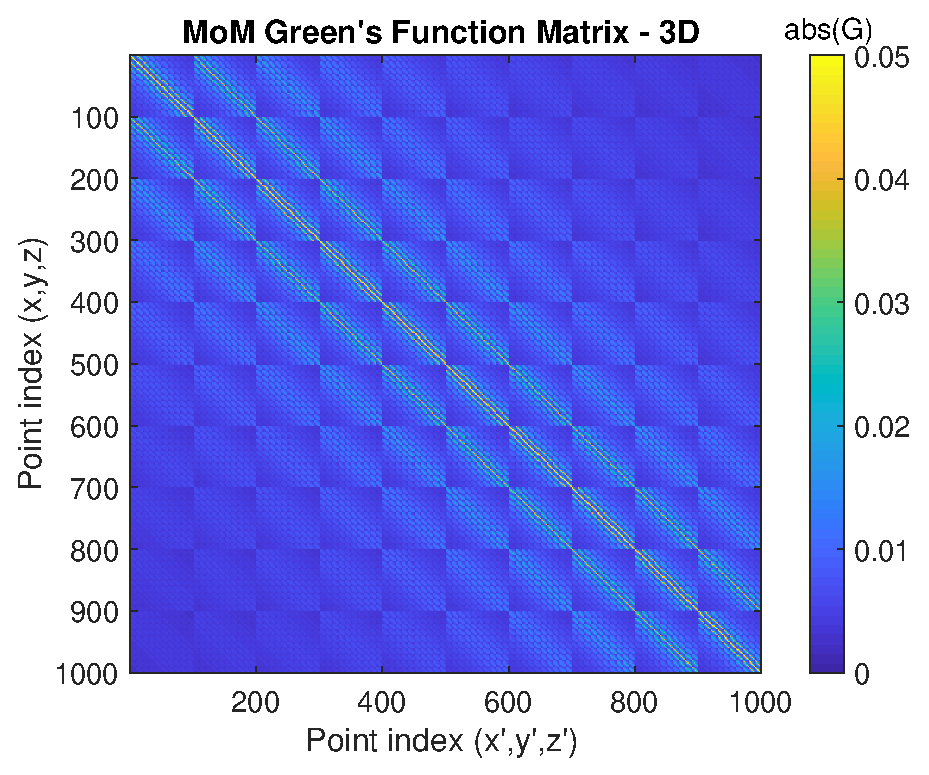
\includegraphics[width=2.5in]{GreensFunctions/Figures/green3d}}
     \subfigure{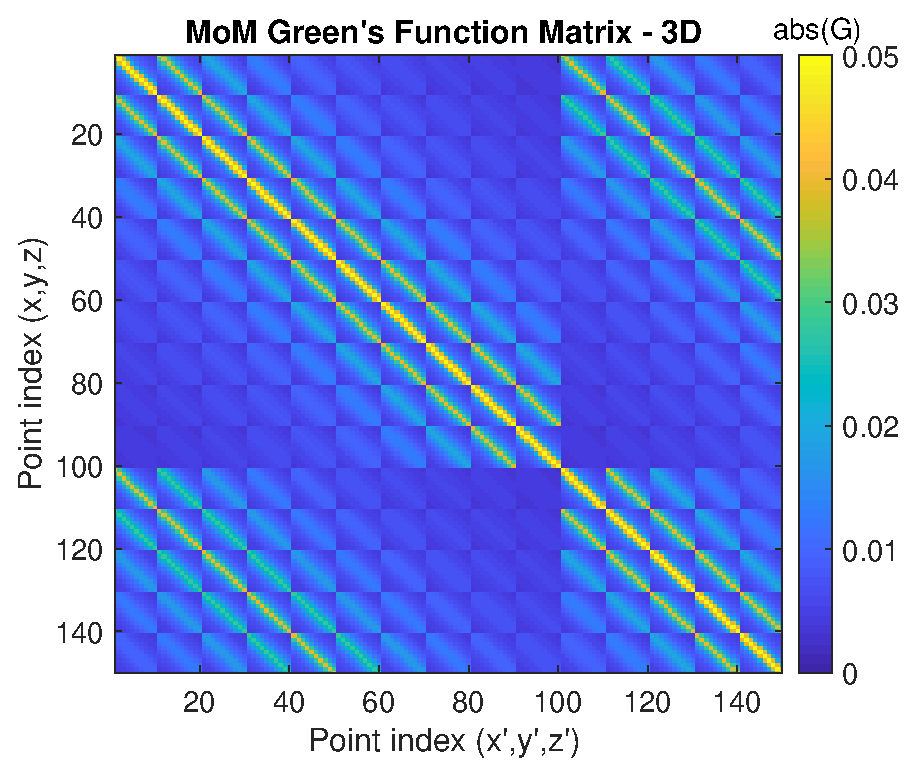
\includegraphics[width=2.5in]{GreensFunctions/Figures/green3d_v2}}
  \end{tabular}
  \label{}
\caption{3D scalar Green's function matrix, $\bb{G}$. Left: full matrix for a 10 $\times$ 10 $\times$ 10 grid of points sampled at $\lambda/5$ (total size of $2\lambda \times 2\lambda \times 2\lambda$). Note, this discretization step is for illustration purposes and is insufficient for an accurate solution. Right: zoom in. The appearance of blocks and subblocks is due to first vectorizing the 3D grid of points, and then taking all possible pairs of interactions which are arranged across rows and columns. For example, the first upper left subblock (sized 10 $\times$ 10), contains the 100 pairs of interactions between the 10 points along one edge of the 3D grid. The diagonal of the matrix are the self terms. }
\end{figure}


\vspace{-5mm}
\paragraph{Routines} The routine \texttt{momGmatrix2D} returns the 2D scalar Green's function matrix for the MoM solution. It takes as input the side length of the square voxel, $\Delta x$, which is assumed constant for all voxels, the background wavenumber $k_b$, and the $(x,y)$ and $(x',y')$ coordinate pairs at which the Green's function will be evaluated. The voxel size length is used to evaluate the volume-integrated singular and non-singular scalar factors which are automatically included in the matrix elements. The arrays of unprimed and primed coordinate pairs can be different sizes: the output matrix is sized $M \times N$ where $M$ is the total number of unprimed points down rows, and $N$ is the total number of primed points across columns. The inputs of primed and unprimed coordinates are separated to facilitate the construction of $\bb{G}$ in subblocks when the number of points is large. If the complete matrix is desired, just input the same arrays for unprimed and primed coordinates, and the routine will return the full square matrix. The points are vectorized column-wise, so the corresponding object function or incident field need to be vectorized column-wise to be consistent. 


{\scriptsize
\VerbatimInput{\code/GreensFunctions/momGmatrix2D.m}
}

\clearpage
The routine \texttt{momGmatrix3D} returns the 3D scalar Green's function matrix for the MoM solution. It takes as input the side length of the cubic voxel, $\Delta x$, which is assumed constant for all voxels, the background wavenumber $k_b$, and the $(x,y,z)$ and $(x',y',z')$ coordinate pairs at which to evaluate the matrix. It otherwise works the same as \texttt{momGmatrix2D}. Because the MoM matrix scales as $O(N^2)$ with the number of 3D voxels, $N$, the total number of elements scales as $O(L^6)$, where $L$ is the side length of a cubic simulation region.



{\footnotesize
\VerbatimInput{\code/GreensFunctions/momGmatrix3D.m}
}



\subsection{Vector MoM}

The vector MoM is derived the same way as the scalar MoM. The major difference is in bookkeeping the vector components and the size of the final matrix. The full vector formulation is needed for any 3D vector scattering problem.  

\paragraph{Total Field}

Starting with the vector VIE, \eqref{vectorVIE}, and substituting the pulse basis function
\eq{\bb{E}(\br) = \bb{E}_{inc}(\br) + \sum_{n}  \int \G{} \cdot O_{n} \delta_{n}(\br') \bb{E}(\br') dV' }

As with the scalar case, the field is assumed constant in each voxel and indexed as
\eq{\bb{E}(\br_m) = \bb{E}_{inc}(\br_m) + \sum_{n}  \int \overline{\bb{G}}(\br_m,\br')  \cdot O_{n} \delta_{n}(\br') \bb{E}(\br_n) dV' }

Assuming Cartesian vector components, $u = (x,y,z)$ and $v = (x,y,z)$, and integrating the dyadic Green's function over the volume-equivalent sphere of the cubic voxel, this is written as a sum for each total field component as
\eq{E_{u,m} = E_{inc,u,m} +  \sum_{v}\sum_{n} G_{uv,mn} O_{n} E_{v,n} \label{Ediscrete} }
\eq{G_{uv,mn} = \begin{cases} G_{uv}(\bb{r}_m,\bb{r}_n) \Delta V, \quad m \neq n\\
G_{uv}(\bb{r}_m=\bb{r}_n), \qquad m = n, u = v \quad (0, u \ne v)  \end{cases}}

\noindent where $\Delta V$ is given by \eqref{voxelint}. The value of the singular integration at the self term, \eqref{singintvec}, is equal to a constant times the identity dyad. The identity dyad means that the self-term only applies to the diagonal elements of the dyad (i.e., $G_{xx}, G_{yy}, G_{zz}$) and is zero for the off-diagonal elements of the dyad. Writing this in matrix notation for the three unknown total field components 
\eq{\left(\bb{I} - \thbth
{\bb{G}_{xx}}{\bb{G}_{xy}}{\bb{G}_{xz}}
{\bb{G}_{yx}}{\bb{G}_{yy}}{\bb{G}_{yz}}
{\bb{G}_{zx}}{\bb{G}_{zy}}{\bb{G}_{zz}} 
\thbth{\bb{O}}{}{}{}{\bb{O}}{}{}{}{\bb{O}}  \right) \thrcol{\bb{E}_x}{\bb{E}_y}{\bb{E}_z} = \thrcol{\bb{E}_{inc,x}}{\bb{E}_{inc,y}}{\bb{E}_{inc,z}} \label{mommatrixtot}}

\noindent where $\bb{I}$ is the identity matrix, $\bb{G}_{uv}$ is the Green's function matrix block for a given polarization pair, $\bb{E}_{inc,v}$ and $\bb{E}_{v}$ are vectors of the incident field and total field solution, respectively, $\bb{O}$ is the diagonal matrix of the object function which is applied to each component. The self term (diagonals) of $\bb{G}_{xx}, \bb{G}_{yy}, \bb{G}_{zz}$, take the value, \eqref{singintvec}, while the self terms of the other blocks are zero. Recall, $\bb{G}_{uv} = \bb{G}_{vu}$, and each block matrix is square symmetric. The size of each block matrix and field vector is the same size as the scalar case. The field components lead to 3 times as many unknowns as compared to the scalar cases, and polarization mixing makes the MoM matrix 9 times larger than the 3D scalar case. 


\paragraph{Induced Current}

Define the induced current as the product of the contrast and the total field at a given point
\eq{ \bb{J}(\br)  =  O(\br) \bb{E}(\br)}

Then \eqref{mommatrixtot} can be written 
\eq{\left(\thbth{\bb{O}^{-1}}{}{}{}{\bb{O}^{-1}}{}{}{}{\bb{O}^{-1}}  - \thbth
{\bb{G}_{xx}}{\bb{G}_{xy}}{\bb{G}_{xz}}
{\bb{G}_{yx}}{\bb{G}_{yy}}{\bb{G}_{yz}}
{\bb{G}_{zx}}{\bb{G}_{zy}}{\bb{G}_{zz}} 
 \right) \thrcol{\bb{J}_x}{\bb{J}_y}{\bb{J}_z} = \thrcol{\bb{E}_{inc,x}}{\bb{E}_{inc,y}}{\bb{E}_{inc,z}}  }


\begin{figure}[H] 
   \centering
      \begin{tabular}{cc}
     \subfigure{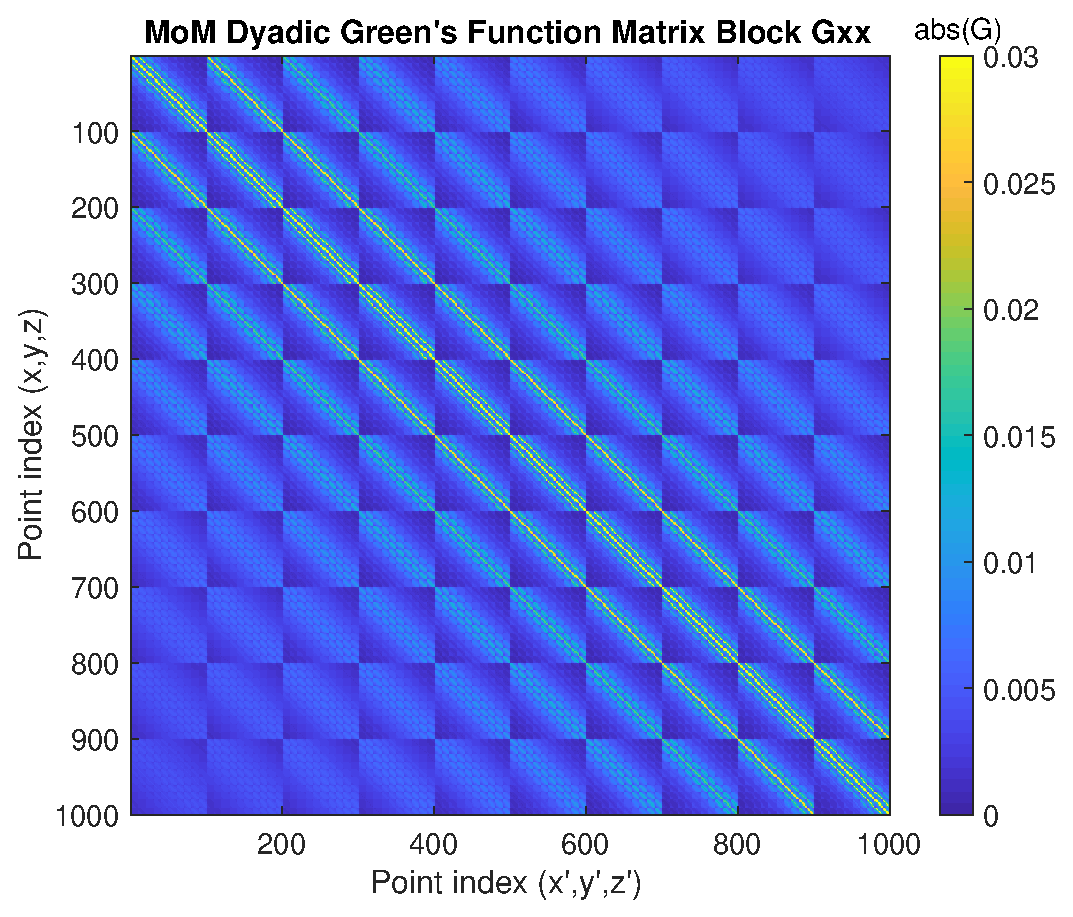
\includegraphics[width=1.9in]{GreensFunctions/Figures/green3dyadic1}}
     \subfigure{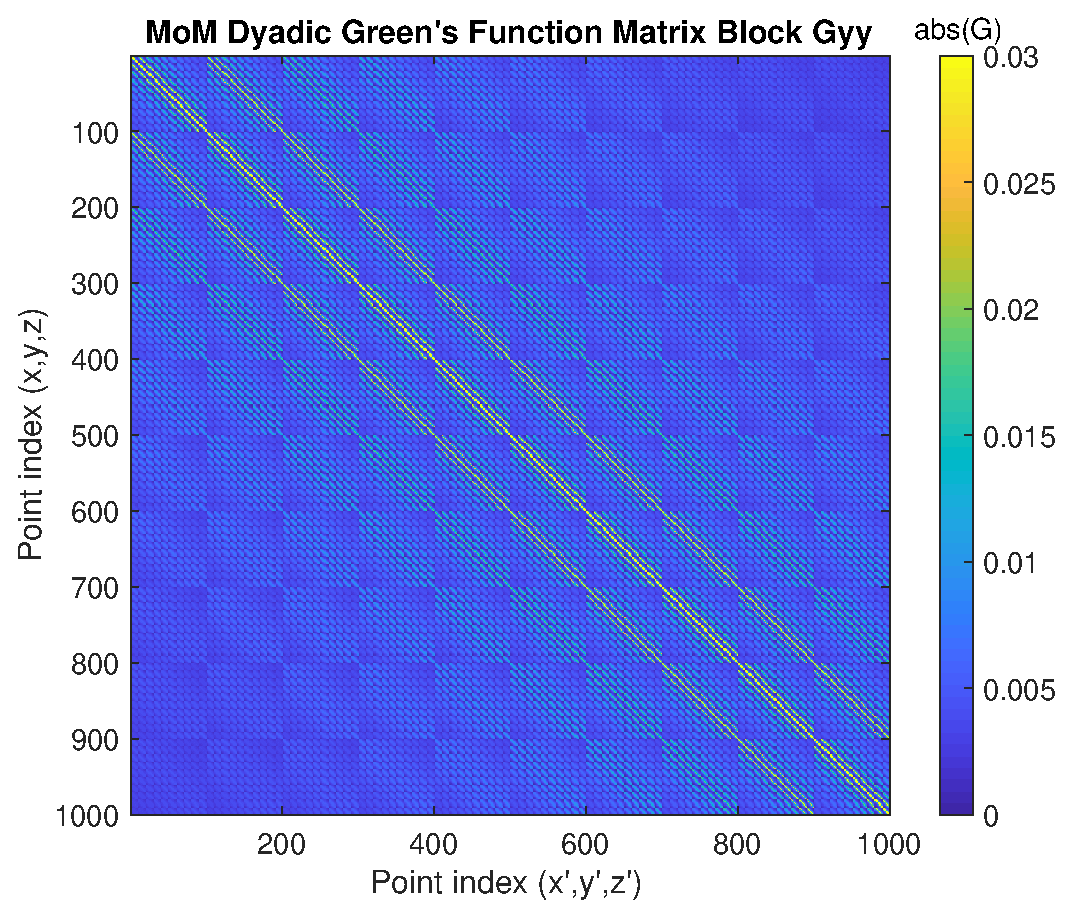
\includegraphics[width=1.9in]{GreensFunctions/Figures/green3dyadic2}} 
     \subfigure{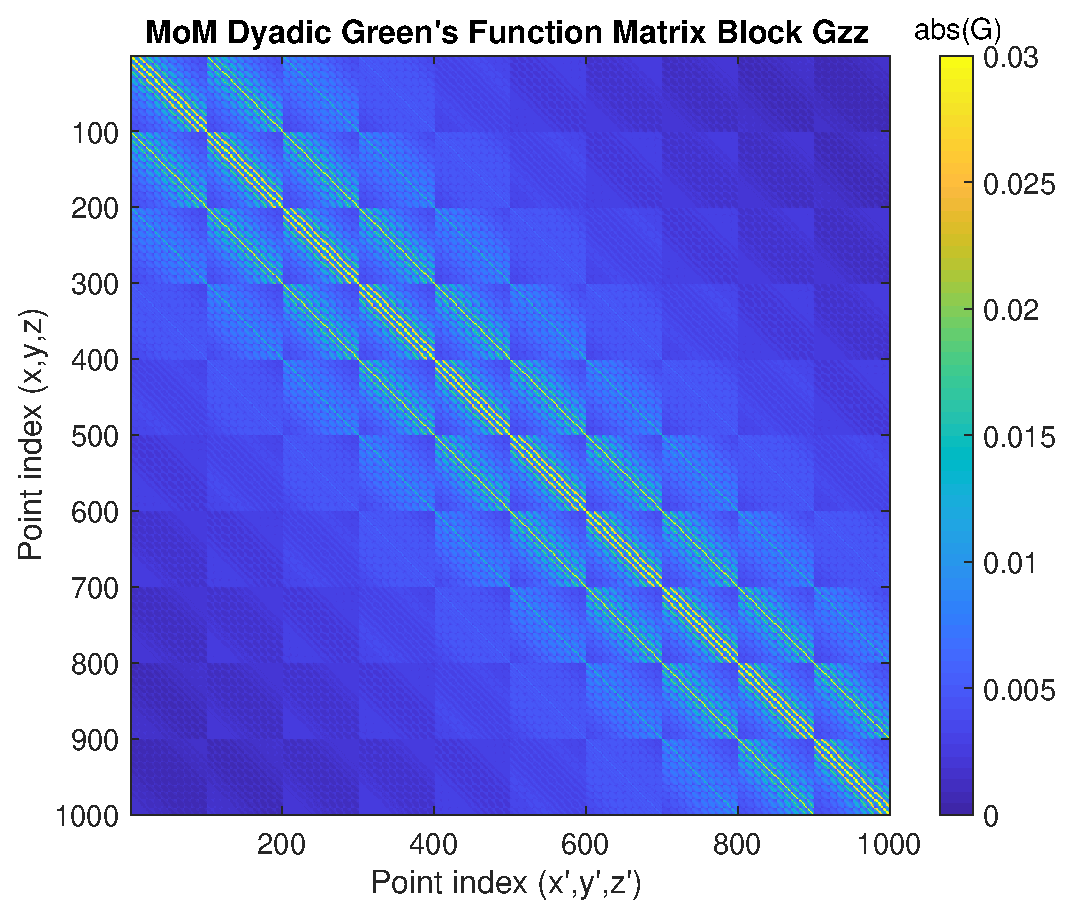
\includegraphics[width=1.9in]{GreensFunctions/Figures/green3dyadic3}} \\
     \subfigure{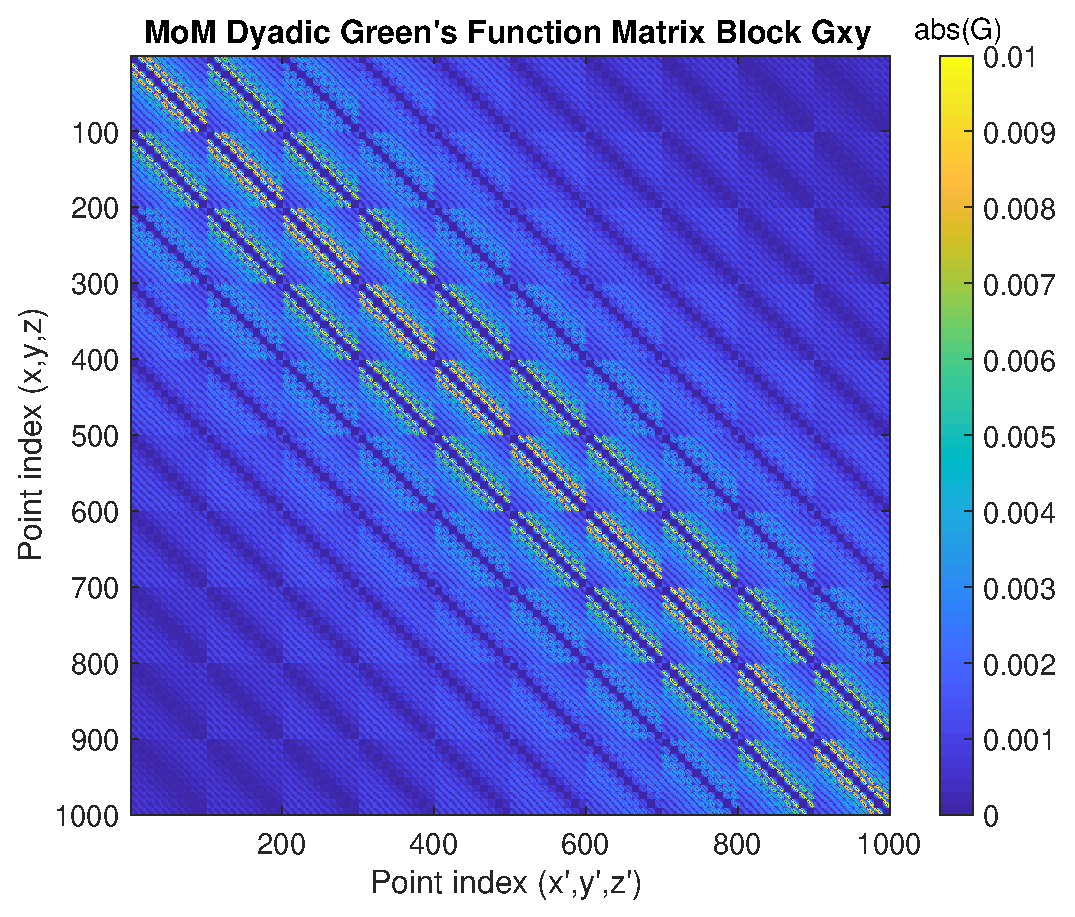
\includegraphics[width=1.9in]{GreensFunctions/Figures/green3dyadic4}} 
     \subfigure{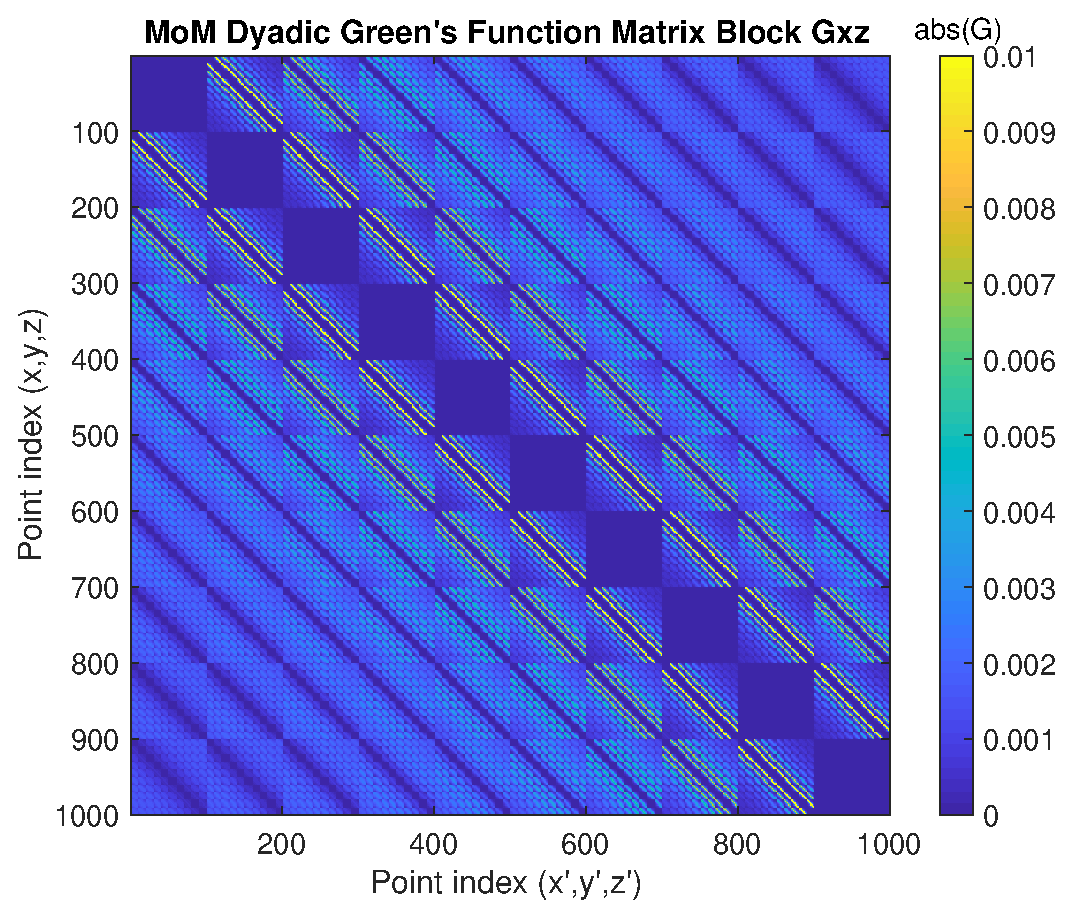
\includegraphics[width=1.9in]{GreensFunctions/Figures/green3dyadic5}}
     \subfigure{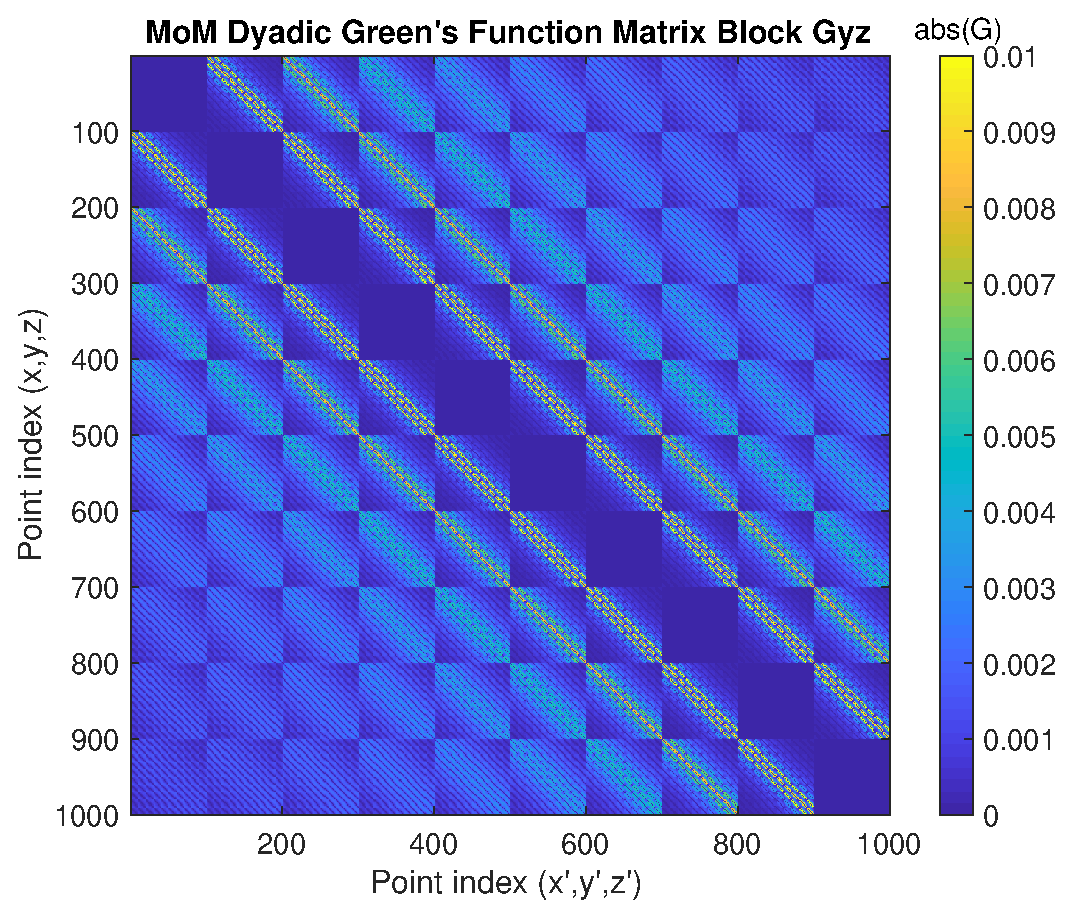
\includegraphics[width=1.9in]{GreensFunctions/Figures/green3dyadic6}}
  \end{tabular}
  \label{}
\caption{3D dyadic Green's function block matrices, $\bb{G}_{uv}$. Full block matrices for a 10 $\times$ 10 $\times$ 10 grid of points sampled at $\lambda/5$ (total size of $2\lambda \times 2\lambda \times 2\lambda$). The zero elements in $\bb{G}_{u \ne v}$ happen when voxels have common coordinates in either $u$ or $v$. This is a result of $\bb{G}_{u \ne v}$ being proportional to the difference of primed and unprimed coordinates in $u$ or $v$. }
\end{figure}

\paragraph{Routine} The routine \texttt{momGmatrixDyadic} returns the 6 unique block matrices of the 3D dyadic MoM matrix.  It takes as input the side length of the cubic voxel, $\Delta x$, which is assumed constant for all voxels, the background wavenumber $k_b$, and the $(x,y,z)$ and $(x',y',z')$ coordinate pairs at which to evaluate the matrix. It works similarly to \texttt{momGmatrix2D} and \texttt{momGmatrix3D}, but calls \texttt{dyadicGreens} which takes the relative positions as input. The arrays of unprimed and primed coordinate pairs can be different sizes. The output matrix is sized $M \times N$ where $M$ is the total number of unprimed points down rows, and $N$ is the total number of primed points across columns. In the routine, the volume integrated constants are applied to all entries. The singularity constant is applied to the self terms of the blocks $\bb{G}_{u = v}$, while the self terms of the blocks $\bb{G}_{u \ne v}$ are set to zero. 



{\footnotesize
\VerbatimInput{\code/GreensFunctions/momGmatrixDyadic.m}
}

\clearpage
\newpage

\section{Scattered Field VIE}

Once the total field solution is found, the scattered field away from the object is computed again with the VIE. Here, the unprimed position vector of the Green's function is evaluated at an observation point outside of the object domain. In this case, the Green's function is often referred to as the receiver Green's function. This can be a point of confusion when comparing it to the Green's function as used in the MoM solution, where the unprimed position vector is evaluated throughout the object domain including at singular points. In the end, the receiver Green's function is the same as the one used in the MoM solution, except that the unprimed position vector is simply evaluated outside of the object at a point that is also usually associated with a sensor.

From reciprocity, it turns out that the receiver Green's function is equivalent to the incident field generated by a point source at the observation location. This is practically and conceptually useful. It links the incident field needed when solving for the total field solution to the scattered field VIE needed to compute the measurements from sources or receivers at the same location. This idea is generalized to the case of real antennas fed by waveguides using the waveport vector Green's function described in \cite{haynes2012vector}. The overarching idea here is that only the incident field of a source or an antenna needs to be known in order to compute both the total field solution and the received voltage measurements in a consistent way. 

\subsection{Receiver Green's Function}
\paragraph{Scalar case}
Let a source be at location $\br_i$. This generates an incident field, $\phi_{inc,i}(\br)$, for which the total field solution in the object is $\phi_{i}(\br)$. The scattered field observed at a point, $\br_j$, outside the object is
\eq{\phi_{sca,ji}(\br_j) = \int g(\br_j,\br') O(\br') \phi_i(\br') dV', \qquad \br_{j} \notin V \label{scalarscaji}}

\noindent where, $g(\br_j,\br')$ is the receiver Green's function. The receiver Green's function is named this way because the unprime variable is evaluated at the receiver, or observation, point. This VIE is discretized the same way as the MoM: the Green's function is integrated over volume-equivalent voxels so that
\eq{\phi_{sca,ji}(\br_j) \approx \Delta V \sum_{n} g(\br_j,\br_n) O(\br_n) \phi_i(\br_n) \label{scalarscadiscrete}}
 
\noindent where $\Delta V$ is given by \eqref{voxelint} in the 3D case. Because $\br_{j} \notin V$, there is no singular point to deal with.

\paragraph{Vector case}

Let a vector source, like an antenna, be located at $\br_i$. This generates an incident field, $\bb{E}_{inc,i}(\br)$, for which the total field solution in the object is $\bb{E}_{i}(\br)$. The scattered field observed at a point, $\br_j$, outside the object is
\eq{\bb{E}_{sca,ji}(\br_j)=  \int \overline{\bb{G}}(\br_j,\br')\cdot O(\br') \bb{E}_i(\br') dV', \qquad \br_{j} \notin V \label{vectorscaji} }

Here, $\overline{\bb{G}}(\br_j,\br')$ is the dyadic receiver Green's function. Discretized like the MoM, this is 
\eq{\bb{E}_{sca,ji}(\br_j) \approx   \Delta V\sum_{n}  \overline{\bb{G}}(\br_j,\br_n)  \cdot O(\br_n) \bb{E}_i(\br_n) \label{vectorscadiscrete} }

\noindent where $\Delta V$ is given by \eqref{voxelint}, there is no singular point, and the dyadic Green's function is evaluated normally. 

\subsection{Incident Field Reciprocity}

The receiver Green's function is equivalent to the incident field generated by a point source at the receiver location when used in transmit mode. This is a consequence of the definition of the Green's function and reciprocity. The derivation is simple, but the idea has important implications for linking the VIE to measurements in experimental setups. In short, the incident field alone fully characterizes the transmit and receive characteristics of a reciprocal sensor. We derive the results for scalar and vector point sources, but the results hold for arbitrary source distributions. 

\paragraph{Scalar case}

Define a scalar point source at location $\br_j$ as $s(\br) = -\delta(\br - \br_j)$. Using \eqref{sourceintscalar}, the incident field from this source is
\ea{\phi_{inc,j}(\br) &=&  -\int g(\br,\br') s(\br') dV' \\
\ &=& \int g(\br,\br') \delta(\br' - \br_j) dV' \\
\ &=&  g(\br,\br_j) }

This is another way of stating the definition of the Green's function. Using the fact that $g(\br,\br_j) = g(\br_j,\br)$, and substituting this into \eqref{scalarscaji}, the scattered field VIE is
\eq{\phi_{sca,ji}(\br_j) = \int \phi_{inc,j}(\br') O(\br') \phi_i(\br') dV' \label{scalarscajiinc}}

The incident field from the point source takes the place of the receiver Green's function. From linearity, this holds for an incident field from an arbitrary source distribution so long as the same device is used as the receiver. Finally, \eqref{scalarscajiinc} is discretized the same as \eqref{scalarscadiscrete}. 

\paragraph{Vector case}

Let the current source be an infinitesimal dipole at $\br_j$ with strength $I$ and polarization $\hat{\bb{p}}$
\eq{\bb{J}(\br) = I \hat{\bb{p}} \delta(\br - \br_j)}

Substituting this into \eqref{evolintj}
\ea{\bb{E}_{inc,j}(\br) &=& i\omega\mu\int \overline{\bb{G}}(\br,\br') \cdot \bb{J}(\br') dV' \\
 \ &=& i\omega\mu I \int \overline{\bb{G}}(\br,\br') \cdot \hat{\bb{p}} \delta(\br' - \br_j) dV'  \\
  \ &=& i\omega\mu I  \overline{\bb{G}}(\br,\br_j) \cdot \hat{\bb{p}} }

or
\ea{ \overline{\bb{G}}(\br,\br_j) \cdot \hat{\bb{p}} = \dfrac{1}{i\omega\mu I }\bb{E}_{inc,j}(\br)  }

A similar expression can be found in \cite{cui2004study} for 2D problems. The columns of the dyadic receiver Green's function are found by computing the incident field due to three orthogonal dipoles in turn. Denote these incident fields $\bb{E}_{inc,j,p}$ for dipole polarizations $p = [x, y, z]$ located at the observation point. Then using the fact that $\overline{\bb{G}}(\br,\br_j) = \left[ \overline{\bb{G}}(\br_j,\br)\right]^{t}$, we have
\eq{ \overline{\bb{G}}(\br_j,\br)  = \dfrac{1}{i\omega\mu I }\cvec{\bb{E}_{inc,j,x}^t(\br)}{\bb{E}_{inc,j,y}^t(\br)}{\bb{E}_{inc,j,z}^t(\br)} \label{incdyad}}

The matrix on the right hand side is denoted the incident field dyad. The transposes place the $[x,y,z]$ vector components of each dipole incident field along the rows of the dyad, which maps the three-vector total field (or induced source) in the domain to the polarizations of the source dipole at the receiver location. Substituting this into \eqref{vectorscaji}, the scattered field VIE for the electric field is
\eq{\bb{E}_{sca,ji}(\br_j)= \dfrac{1}{i\omega\mu I }\int \cvec{\bb{E}_{inc,j,x}^t(\br')}{\bb{E}_{inc,j,y}^t(\br')}{\bb{E}_{inc,j,z}^t(\br')} \cdot O(\br') \bb{E}_i(\br') dV' \label{vectorscajiinc} }

In simulation, one can set $I = 1/i\omega\mu$ to cancel the scale factor and \eqref{vectorscajiinc} can be discretized like \eqref{vectorscadiscrete}. The physical interpretation of \eqref{vectorscajiinc} is the following. The three source dipoles at the observation location independently map to a three-vector incident field in the object domain. Concurrently, each vector component of the induced current in the domain radiates all three vector components to the observation point. The columns of the incident field dyad, \eqref{incdyad}, map any single component of the induced current to the three components at the observation location in proportion to the strength of the incident fields created by the corresponding source dipoles. This is another way of stating reciprocity. %For example, an $x$ directed current in the object radiates all three vector components at the observation point and the weights of this mapping are determined are determined by the $x$ components of each of the three incident fields. The same happens for the other two components to accomplish the full dyadic mixing. 


\subsection{Waveport Vector Green's Function}
When measuring fields with real antennas, we never measure the three electric field components directly. We measure a voltage on a feeding waveguide or transmission line. The three vector components of the scattered field are effectively integrated over the surface of the antenna and produce the voltage on the waveguide. The incident field dyad above collapses to three-vector incident field with certain scale factors. This was formalized in \cite{haynes2012vector} in the form a waveport vector Green's function. The idea is fundamentally the same as the receiver Green's function and incident field dyad, except that it is specialized for S-parameter measurements between two antennas that are made using a vector network analyzer (VNA) with calibrated reference planes on the feeding transmission lines. 

\begin{figure}[H] 
\centering
\includegraphics[width=3in]{GreensFunctions/Figures/SparamVIE}
\caption{Network model of two antennas and a scattering object. $S$-parameters are measured between the reference planes on antenna transmission lines, \cite{haynes2012vector}.}
\label{sparamviefig}
\end{figure}

Let two antennas in frames $i$ and $j$ be used to probe an object with a VNA that measures the entire system as a 2-port device, as shown in Figure \ref{sparamviefig}. The complex excitation amplitudes on each transmission line are $a_o^i$ and $a_o^j$, while the received amplitudes are $b_o^i$ and $b_o^j$. The VNA is calibrated to the reference planes on the transmission lines. Assume that the spatial distribution of the antenna incident field is referenced to a fixed coordinate origin of the antenna, and the excitation (amplitude and phase) is referenced to the calibration planes on the transmission line. The waveport vector Green's function is
\eq{\bb{g}(\br) = -\dfrac{Z_o}{2a_o}\dfrac{1}{i\omega\mu} \bb{E}_{inc}(\br)}

\noindent where $Z_o$ is the characteristic impedance of the receiver transmission line and $a_o$ is the excitation used to create the incident field $\bb{E}_{inc}(\br)$. The waveport vector Green's replaces the dyadic receiver Green's function \eqref{incdyad} and effectively collapses the dyad.
When used in the VIE, the 2-port scattered field $S$-parameter measurement, $S_{ji}$, is given by 
\eq{S_{ji} = -\dfrac{1}{2i\omega\mu} \dfrac{Z_o^j}{a_o^j a_o^i} \int \bb{E}_{inc,j}(\br') \cdot O(\br') \bb{E}_{i}(\br') dV'}

\noindent where $a_o^j$ is the excitation used to create the incident field of the receiver, $\bb{E}_{inc,j}(\br')$, and $a_o^i$ is the excitation used to create the incident field of the transmitter $\bb{E}_{inc,i}(\br')$ which in turn is used to compute the solution of the total field $\bb{E}_{i}(\br')$.  In practice, if we know the average transmit power on the transmission line, $P_{ave}$, then from transmission line analysis the magnitude of $a_o$ is given by 
\eq{\vert a_o \vert = \sqrt{2 Z_o P_{ave}}}

The phase of $a_o$ can be found by comparing the transmission line reference plane used to measure or simulate the incident fields to the reference planes used in measurement. 









